\lecture{4}{16. Februar 2026}{Equilibrium Equations \& Principle of Angular Momentum}

\subsection{Equilibrium}

\subsubsection{Foundations}
The principle of linear momentum is
\begin{equation} \label{eq:linmomprin}
  \int_V \Vec{f} \, \mathrm{d}V + \int_A \Vec{T} \, \mathrm{d}A = \int_V \rho \Vec{\ddot{u}} \, \mathrm{d}V
\end{equation}
where $\rho$ is the mass density and $\Vec{u}$ is the displacement.

The principle of angular momentum is
\begin{equation} \label{eq:angmomprin}
  \int_V \left( \Vec{r} \times \Vec{f} \right) \, \mathrm{d}V + \int_A \left( \Vec{r} \times \Vec{T} \right) \, \mathrm{d}A = \int_V \left( \Vec{r} \times \rho \Vec{\ddot{u}} \right) \, \mathrm{d}V
\end{equation}
where $\Vec{r}$ is the position vector.

We will also utilize the divergence theorem:
\begin{equation} \label{eq:divthe}
  \int_V \nabla \cdot \Vec{G} \, \mathrm{d}V = \int_A \Vec{n} \cdot \Vec{G} \, \mathrm{d}A
.\end{equation}

These can each be written in component form using:
\begin{align*}
  \Vec{f} &= f_i \Vec{e}_i \\
  \Vec{T} &= \sigma_{ji} n_j \Vec{e}_i \\
  \Vec{r} &= x_j \Vec{e}_j \\
  \Vec{r} \times \Vec{f} &= \epsilon_{ijk} x_j f_k \Vec{e}_i \\
  \Vec{r} \times \Vec{T} &= \epsilon_{ijk} x_j \sigma_{lk} n_l \Vec{e}_i
.\end{align*}

For static problems, the rhs of \Cref{eq:linmomprin,eq:angmomprin,eq:divthe} are zero.
Substituting this and using the above component-form we get
\begin{align}
  \int_V f_i \, \mathrm{d}V + \int_A \sigma_{ji} n_j \, \mathrm{d}A &= 0 \label{eq:linmomprincom}\\
  \int_V \epsilon_{ijk} x_j f_k \, \mathrm{d}V + \int_A \epsilon_{ijk} x_j \sigma_{lk} n_l \, \mathrm{d}A &= 0 \label{eq:angmomprincom}\\
  \int_V G_{i,i} \, \mathrm{d}V &= \int_A n_i G_i \, \mathrm{d}A \label{eq:divthecom}
.\end{align}

\subsubsection{Linear Momentum}
If we apply \Cref{eq:divthecom} with $G_i = \sigma_{ji}$ to \Cref{eq:linmomprincom} we get:
\begin{equation*}
  \int_V f_i + \sigma_{ji, j} \, \mathrm{d}V = 0
.\end{equation*}
For all elements of $V$ to be in equilibrium, the above equation is satisfied if the integrand vanishes, i.e.
\begin{equation} \label{eq:linmomres}
  \sigma_{ji,j} + f_i = 0
.\end{equation}
This represents three equilibrium equations in terms of nine unknown components of stress $\sigma_{ij}$.

\subsubsection{Angular Momentum}
We apply \Cref{eq:divthecom} with $G_i = \epsilon_{ijk} x_j \sigma_{lk}$ and $n_i = n_l$ to \Cref{eq:angmomprincom} and get:
\begin{equation} \label{eq:angmom}
  \int_V \epsilon_{ijk} x_j f_k + \left( \epsilon_{ijk} x_j \sigma_{lk} \right)_{,l} \, \mathrm{d}V = 0
.\end{equation}
The second term is expanded as
\begin{equation*}
  \left( \epsilon_{ijk} x_j \sigma_{lk} \right)_{,l} = \epsilon_{ijk} \sigma_{lk} x_{j,l} + \epsilon_{ijk} x_j \sigma_{lk,l}
.\end{equation*}
Also we use that $x_j$ only changes in the $j$'th direction: i.e.
\begin{equation*}
  x_{j,l} = \delta_{jl}
.\end{equation*}
Hence, \Cref{eq:angmom} becomes:
\begin{equation*}
  \int_V \epsilon_{ijk} \left( x_j f_k + \delta_{jl} \sigma_{lk} + x_j \sigma_{lk,l} \right) \, \mathrm{d}V = 0
\end{equation*}
the first and third term combines to
\begin{equation*}
  \epsilon_{ijk} x_j \left( f_k + \sigma_{lk,l} \right) = 0
\end{equation*}
from \Cref{eq:linmomres}.
The remaining term becomes
\begin{equation*}
  \epsilon_{ijk} \delta_{jl} \sigma_{lk} = \epsilon_{ijk} \sigma_{jk}
.\end{equation*}
So the equation reduces to
\begin{equation*}
  \int_V \epsilon_{ijk} \sigma_{jk} \, \mathrm{d}V = 0
\end{equation*}
which holds for
\begin{equation*}
  \epsilon_{ijk} \sigma_{jk} = 0
.\end{equation*}
In general, this is satisfied for
\begin{equation*}
  \sigma_{ij} = \sigma_{ji}
.\end{equation*}

This allows us to rewrite the component definition of traction as
\begin{equation*}
  T_i = \sigma_{ij} n_j
\end{equation*}
and \Cref{eq:linmomres} as
\begin{equation*}
  \sigma_{ij,j} + f_i = 0
.\end{equation*}
Which corresponds to the statically indeterminate system:
\begin{align*}
  \sigma_{11,1} + \sigma_{12,2} + \sigma_{13,3} + f_1 &= 0 \\
  \sigma_{21,1} + \sigma_{22,2} + \sigma_{23,3} + f_2 &= 0 \\
  \sigma_{31,1} + \sigma_{32,2} + \sigma_{33,3} + f_3 &= 0
.\end{align*}


\subsection{Principal Stress}

\subsubsection{Definition and Derivation}
We consider the normal section through a body shown on \Cref{fig:f2_6a}.
The traction $\Vec{T}_n$ acts on the plane defined by $\Vec{n}$ that appears edgewise.

\begin{figure} [ht]
  \begin{subfigure}{0.58\linewidth}
    \centering
    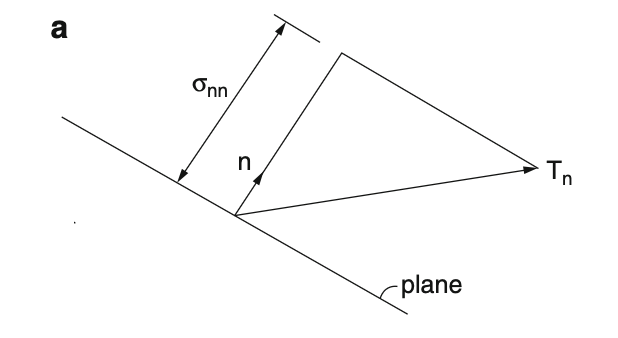
\includegraphics[width=0.8\linewidth]{./figures/f2_6a.png}
    \caption{Normal section}
    \label{fig:f2_6a}
  \end{subfigure}
  \begin{subfigure}{0.38\linewidth}
    \centering
    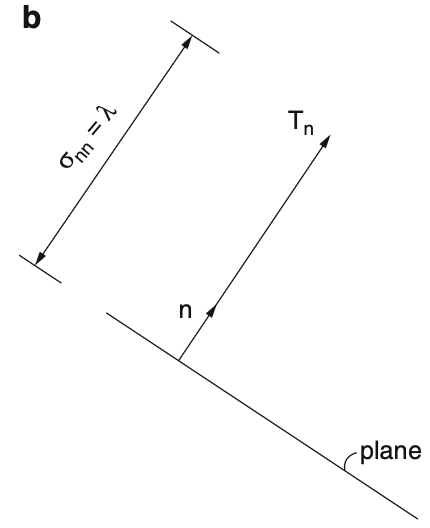
\includegraphics[width=0.8\linewidth]{./figures/f2_6b.png}
    \caption{Principal plane}
    \label{fig:f2_6b}
  \end{subfigure}
\end{figure}

Using the dyadic form,
\begin{equation*}
  \sigma_{nn} = \Vec{T}_n \cdot \Vec{n} = \Vec{\sigma} \cdot \Vec{n} \cdot \Vec{n}
\end{equation*}
we seek the orientation of a plane, given by $\Vec{n}$, such that $\sigma_{nn}$ is an extremum.
Such a plane is called a \textit{principal} plane.

Hence,
\begin{align*}
  \frac{\mathrm{d}\sigma_{nn}}{\mathrm{d}n} &= \Vec{n} \cdot \frac{\mathrm{d}(\Vec{\sigma} \cdot \Vec{n})}{\mathrm{d}n} + (\Vec{\sigma} \cdot \Vec{n}) \cdot \frac{\mathrm{d}\Vec{n}}{\mathrm{d}n} \\
  &= 2 (\Vec{\sigma} \cdot \Vec{n}) \cdot \frac{\mathrm{d}\Vec{n}}{\mathrm{d}tn}  \\
  &= 2 \Vec{T}_n \cdot \frac{\mathrm{d}\Vec{n}}{\mathrm{d}n}  \\
  &= 0
.\end{align*}

For $\Vec{T}_n \cdot \frac{\mathrm{d}\Vec{n}}{\mathrm{d}n}$ to equal 0, $\Vec{T}_n$ must be normal to $\frac{\mathrm{d}\Vec{n}}{\mathrm{d}n}$.
Furthermore, $\frac{\mathrm{d}\Vec{n}}{\mathrm{d}n} $ is normal to $\Vec{n}$, so $\Vec{T}_n$ must be parallel to $\frac{\mathrm{d}\Vec{n}}{\mathrm{d}n}$.
This condition corresponding to the extremum is shown in \Cref{fig:f2_6b}.
Here, the tangential component $\sigma_{ns} = 0$ and the normal component for this case is designated as
\begin{equation*}
  \sigma_{nn} = \left| \Vec{T}_n \right| = \lambda
\end{equation*}
which may also be represented as
\begin{equation*}
  \Vec{T}_n = \lambda \Vec{n}
\end{equation*}
or in component form as
\begin{equation*}
  T_i = \lambda n_i
.\end{equation*}
Also, we know that
\begin{equation*}
  T_i = \sigma_{ji} n_j
.\end{equation*}

Equating these gives
\begin{equation*}
  \lambda n_i = \lambda n_j \delta_{ij} = \sigma_{ji} n_j
\end{equation*}
or
\begin{equation} \label{eq:prinor}
  \left( \sigma_{ji} - \lambda \delta_{ij} \right) n_j = 0
.\end{equation}
This is a set of three equations in four unknowns, $n_1, n_2, n_3,$ and $\lambda$.
The components $n_j$ determine the orientation of the principal plane and $\lambda$ is the principal stress.
This is a linear eigenvalue problem, and with Cramer's rule, it can be shown that a nontrivial solution may be found if the determinant of the coefficients of $n_j$ vanishes, i.e.
\begin{equation*}
  \left| \sigma_{ji} - \lambda \delta_{ij} \right| = 0
\end{equation*}
or
\begin{equation*}
  \begin{vmatrix}
    \sigma_{11}-\lambda & \sigma_{12} & \sigma_{13}\\
  \sigma_{21} & \sigma_{22}-\lambda & \sigma_{23}\\
  \sigma_{31} & \sigma_{32} & \sigma_{33}-\lambda\\
  \end{vmatrix} = 0
.\end{equation*}

This expands into a cubic equation for $\lambda$ indicating that three principal stresses, $\lambda_1 = \sigma^{(1)}, \lambda_2 = \sigma^{(2)}, \lambda_3 = \sigma^{(3)}$, exist.
For each principal stress, a corresponding distinct principal orientation may be evaluated by substituting, a known value of $\sigma^{(k)}$ into \Cref{eq:prinor}.
As this still represents three equations in four unknowns, the additional supplementary relationship:
\begin{equation*}
  n_j^{(k)} n_j^{(k)} = 1
\end{equation*}
expressing the ``length'' of the unit normal for $k = 1,2,3$ must also be introduced. 


\subsection{Properties and Special States of Stress}

\subsubsection{Plane Stress}
Consider a plane passing through $P$ with no stresses, i.e. $\Vec{T} = 0$.
The projection theorem states that the traction on any other plane passing through $P$ must be perpendicular to the normal to the stress-free plane; hence, it is parallel to that plane.
Consequently, if the traction on a plane is parallel to another plane, then the latter plane will be stress free.
This is known as a state of \textit{plane stress} and is of practical use since this allows us to reduce the dimensionality of elasticity problems.

If one of the principal stresses is zero, the state of stress is plane.

\subsubsection{Linear Stress}
For two nonparallel planes on which $\Vec{T} = 0$, the traction on any other plane must be parallel to both of these planes and also to their line of intersection.
This is a state of \textit{linear stress} and is essentially a one-dimensional problem, where two principal stresses vanish.

\subsubsection{Pure Stress}
If, for any coordinate system
\begin{equation*}
  \sigma_{11} = \sigma_{22} = \sigma_{33} = 0
\end{equation*}
the state of stress is called \textit{pure shear} since only shear stresses, $\sigma_{ij}, i \neq j$ exist.
For pure shear, $\sigma_{ii} = 0$ for any coordinate system.

\subsubsection{Hydrostatic Stress}
If the principal stresses $\sigma^{(1)}$ are all equal, then the stress state is hydrostatic, and the shearing stresses are zero.
